\section{Real-Data Study: Geometry, Dynamics, and Scope}
\label{sec:real}

The synthetic experiments in Section~\ref{sec:experiments} verify the
theorems where their assumptions hold. This section takes the theory to
a production-scale spectral-spatial pipeline: per-pixel 4-class tissue
classification on QCL infrared hyperspectral images of breast cancer
tissue microarrays. It contains two kinds of evidence with two distinct
roles. First, a production-scale \emph{observation} from a companion
empirical study \citep{dziuba2026spatial}: end-to-end training of the
spectral module loses badly to pretraining and freezing it. Second, a
\emph{controlled, instrumented study} on the same data and architecture
family, designed to test the theorems' predictions directly --- with
matched arms, logged gradient dynamics, and the optimizer family varied
across momentum SGD and AdamW. The picture that emerges is more
qualified than simple confirmation: the block-scalar reading of
Theorem~\ref{thm:hessian} does \emph{not} manifest at initialization,
for a reason we can measure (rank-one input statistics); a strong
directional curvature anisotropy is measurable at initialization,
and whether it starves learning is a hypothesis we state and test; the
momentum-SGD controls, which vary the optimizer family but do not
instantiate Theorem~\ref{thm:twoscale}'s gradient flow, show no
resolvable best-validation difference between joint and frozen arms at
three seeds; and the joint-versus-frozen comparison turns out to depend
on the training
protocol rather than on the architecture --- under our original
protocol it inverts between checkpoint policies, and under a protocol
that equalizes the incidental asymmetries between the arms neither a
freezing benefit nor a freezing penalty is resolvable at three seeds.

\subsection{Pipeline and capacity}
\label{sec:real_setup}

The data are $336 \times 336$ pixel cores collected by QCL
spectroscopy over the $1000$--$1800$~cm$^{-1}$ fingerprint region.
Each pixel carries an $S = 942$ dimensional spectrum (after stacking
raw absorbance and its first two derivatives). The classification
target is per-pixel tissue type. The compositional model is the Block
Vision Transformer of O'Leary et al.~\cite{oleary2026spatial}: a
linear per-pixel $f_\thetap: \R^{942} \to \R^{K}$, then $16 \times 16$
patch tokenization, a 12-layer / 12-head Vision Transformer of
embedding width $M = 192$, a transposed-convolution decoder, and a
convolutional segmentation head. Parameter counts obtained directly
from the instantiated model are given in Table~\ref{tab:capacity}.

\begin{table}[h]
\centering
\caption{Module capacities of the BlockViT-v2 pipeline, counted from
the instantiated model. $K$ is the spectral bottleneck width; the two
rows are the two configurations used in the companion's production
runs.}
\label{tab:capacity}
\begin{tabular}{lrrr}
\toprule
Configuration & $\Cf$ & $\Cg$ & $\Cg/\Cf$ \\
\midrule
$K = 64$ (end-to-end baseline) & $61{,}108$ & $18{,}271{,}540$ & $299$ \\
$K = 128$ (matched to frozen variants) & $121{,}588$ & $21{,}472{,}564$ & $177$ \\
\bottomrule
\end{tabular}
\end{table}

\paragraph{Channel convention.}
O'Leary et al.'s original BlockViT operates on the second-derivative
spectrum alone (a single channel, $S = 965$ for their prostate FTIR
data)---the field-standard preprocessing in infrared histopathology.
The companion benchmark, and hence the models analyzed here, instead
stacks raw absorbance with its first two derivatives (three channels,
$S = 942$). The choice affects only $\Cf$: instantiating the same
model on the single-channel field-standard input gives
$\Cf = 20{,}916$ and $\Cg/\Cf \approx 874$. The three-channel
convention is therefore the \emph{conservative} choice for this
paper's purposes---under the field standard, the capacity asymmetry
we analyze is roughly three times larger.

The capacity ratio is thus roughly two orders of magnitude, and the
spatial module's dominant blocks---the transformer
($5.34 \times 10^6$) and the transposed convolution
($9.44 \times 10^6$)---are both $\Theta(M^2)$ in the embedding width.

\paragraph{The architecture does not satisfy Theorem~\ref{thm:hessian}'s
head hypothesis.}
That $\Theta(M^2)$ scaling is not sufficient to place the model inside
the theorem. BlockViT-v2's segmentation head is the chain
$\mathrm{Conv}_{3\times3}(M{+}K \to 96) \to \mathrm{BN} \to
\mathrm{ReLU} \to \mathrm{Conv}_{3\times3}(96 \to 48) \to \mathrm{BN}
\to \mathrm{ReLU} \to \mathrm{Conv}_{3\times3}(48 \to 4)$, so the final
affine classifier sees $48 \times 3 \times 3 = 432$ input features at
\emph{every} width we build ($M \in \{48,192,384\}$,
$K \in \{64,128\}$): the $\Theta(M)$ feature map is separated from the
logits by two nonlinearities. Theorem~\ref{thm:hessian} requires a
dense classifier head over penultimate features of dimension
$\Theta(M)$ with no downstream nonlinearity
(Lemma~\ref{lem:phi_scaling}), and that hypothesis is therefore not
satisfied here; the $\Cg = \Theta(M^2)$ form of the statement is a
change of variables conditional on the same hypothesis, not an
independent sufficient condition. The theorem's lower bound on the
curvature disparity consequently does not apply as stated to this
model. This is different from the theorem being contradicted: failing a
hypothesis removes a guarantee, it does not reverse the conclusion.
Whether the curvature disparity the theorem permits actually manifests
at initialization is an empirical question, which we now measure
directly.

\subsection{Production-scale observation}
\label{sec:real_observation}

The companion study trains the full pipeline under 5-fold
cross-validation on breast QCL data and reports held-out test macro-F1
for an end-to-end learned linear spectral module against three
pretrain-and-freeze variants (its Table~6):

\begin{table}[h]
\centering
\begin{tabular}{lc}
\toprule
Variant & Test F1 (5-fold mean $\pm$ sd) \\
\midrule
End-to-end learned linear (joint)          & $0.675 \pm 0.036$ \\
Frozen pretrained spectral (Peak Windows)  & $0.842 \pm 0.121$ \\
Frozen pretrained spectral (MLP)           & $0.896 \pm 0.092$ \\
Frozen pretrained spectral (Sliding Win.)  & $0.954 \pm 0.020$ \\
\bottomrule
\end{tabular}
\caption{Held-out test F1 on breast QCL tissue cores, as published in
the companion study \citep{dziuba2026spatial}. End-to-end training of
the spectral module underperforms every pretrain-and-freeze variant by
$0.17$--$0.28$ F1.}
\label{tab:real}
\end{table}

Two remarks on scope. First, this is an \emph{observation that
motivates the controlled study below}, not a theorem test: the
variants differ in both stability (frozen vs.\ jointly trained) and
informativeness (pretrained vs.\ learned from scratch), and the
production runs log no gradient dynamics. Second, the theorems do not
guarantee that pretrain-and-freeze wins. Theorem~\ref{thm:twoscale}
bounds how far the spectral module moves along the \emph{joint}
trajectory in its regime; it does not by itself bound the performance
gap to a separately trained frozen model, and pretraining is a
separate, empirically supported escape route. The controlled study
below examines exactly these factors.

\subsection{Geometry at initialization}
\label{sec:real_geometry}

We measure the Gauss--Newton blocks of the instantiated pipeline on
real training batches at random initialization (Lanczos with full
reorthogonalization on matrix-free GGN block operators, validated to
$10^{-12}$ against dense computation; Section~\ref{sec:experiments}),
sweeping the ViT embedding width $M \in \{48, 96, 192, 384\}$ with
3 seeds $\times$ 4 batches per width.

\paragraph{The block-scalar disparity does not manifest.}
At production width $M=192$ the measured curvature ratio is
$\mathcal{D}_{\mathrm{curv}} = \lambda_{\max}(G_{\phip\phip})/\lambda_{\max}(G_{\thetap\thetap})
= 0.46 \pm 0.21$ --- the \emph{spectral} block carries the larger top
curvature, the opposite of the naive block-scalar expectation. The
ratio rises with width ($0.33 \pm 0.12$ at $M{=}48$ to
$0.70 \pm 0.19$ at $M{=}384$; on prostate QCL it reaches parity,
$1.09 \pm 0.52$, at $M{=}384$) but the disparity regime is nowhere in
sight at buildable widths. The two width-scalings behave differently.
The spectral cap is width-independent, as Theorem~\ref{thm:hessian}
requires (log-log slope of $\lambda_{\max}(G_{\thetap\thetap})$ vs.\ $M$:
$-0.003$ breast, $-0.012$ prostate). The spatial curvature grows, but
sublinearly: the log-log slope of $\lambda_{\max}(G_{\phip\phip})$ vs.\
$M$ is $0.38$ (breast) and $0.45$ (prostate), i.e.\ $115 \to 258$
across an $8\times$ width increase, well short of the $\Omega(M)$
growth of Lemma~\ref{lem:phi_scaling}. That $\Omega(M)$ floor is
neither observed here nor, given the head hypothesis failure noted in
Section~\ref{sec:real_setup}, guaranteed for this architecture.

\paragraph{What carries the width trend.}
The sublinear growth of $\lambda_{\max}(G_{\phip\phip})$ is measurable at
initialization, and it is not the mechanism of
Lemma~\ref{lem:phi_scaling}. In BlockViT-v2 the only downstream layer
whose input dimension grows with $M$ is the first head convolution, and
the second-moment matrix of the (patch-unfolded) features entering it is
flat in $M$: its top eigenvalue is unchanged to four significant figures
across $M \in \{48, 192, 384\}$ (3 seeds), with the leading direction
inside the width-independent $K{=}64$ skip channels. At initialization,
the positive width trend in the decoder's spatial GGN is sensitive to head
batch normalization: using fixed initial statistics in the two head BNs
removes the trend while preserving the incoming features (pooled log-log
slope of the first-convolution block's top curvature: $+0.61$ with batch
statistics, per seed $+0.35$ to $+0.79$; $+0.006$ with both head BNs at
their initial running statistics, per seed $-0.11$ to $+0.18$; whole
$\phip$ block $+0.40 \to -0.33$), and either BN alone carries it ($+0.56$
and $+0.57$). The mechanism is a normalization gain on width-diluted
activations. Under fan-in initialization the per-channel pre-BN variance
of the first head BN falls as $1/(M{+}K)$ ($0.15, 0.064, 0.035$ at the
three widths; medians over channels, 3 seeds), because the fan-in grows
with $M$ while the incoming energy sits almost entirely in the
width-independent skip channels; the BN's inverse-standard-deviation gain
grows correspondingly ($2.6, 4.0, 5.4$), so a unit weight perturbation
whose pre-BN energy is width-independent leaves the BN with energy growing
roughly as $M^{1/2}$ (measured slopes $0.46$--$0.56$) and reaches the loss
as $M^{0.6}$. A spatially constant bias perturbation is annihilated
exactly. A function-preserving rescaling of that convolution (weights and
bias by $c$, BN stabilizer by $c^2$) leaves every logit unchanged and
scales the block's top curvature by exactly $c^{-2}$ (measured $1.0000$
for $c \in \{\tfrac14, \tfrac12, 2, 4\}$), so the raw Euclidean curvature
of a layer that feeds a batch normalization is a parameterization
quantity, not an architectural one \citep{vanlaarhoven2017l2}. This sweep
therefore does not validate the width-linear feature-Gram mechanism of our
shallow theory, and we do not use it as architectural evidence. Slopes
over three widths are descriptive; the interventions establish
sensitivity, not a unique cause, since switching a BN to fixed statistics
also changes its forward output and the gates downstream of it. The
denominator, by contrast, we can diagnose directly.

\paragraph{Diagnosis: rank-one input statistics.}
The input second-moment matrix $\Sigma_X$ of real tissue spectra has
effective rank $1.07$ (breast) and $1.02$ (prostate) out of $942$ on
the raw inputs; measured after the module's input batch normalization
the same quantity is $1.21$ (breast), so the near-rank-one structure is
a property of the spectra and not an artifact of the normalization.
Every tissue spectrum shares the same dominant mean shape, and the cap
$C_\theta \propto \lambda_{\max}(\Sigma_X)$ is correspondingly enormous.
Theorem~\ref{thm:hessian}'s disparity bound is not established for this
model (its head hypothesis fails); independently, rank-one inputs make
the cap side uninformative: even where the bound applies, it constrains
nothing at buildable widths, because the data concentrate almost all
their second-moment mass in one direction. This is a regime in which
the scalar bound is uninformative, not a counterexample: the theorem's
disparity is a statement about what capacity \emph{permits}, and
rank-one inputs hand the spectral block a single direction of huge
curvature.

\paragraph{Directional curvature anisotropy.}
Because the spectral curvature is rank-deficient, the block-scalar
ratio is the wrong lens; restricting the GGN to individual directions
reveals an anisotropy the scalar hides. Write $v_1$ for the leading
eigenvector of the post-normalization input second-moment matrix; it
coincides with the mean-spectrum direction ($|\cos| > 0.995$
post-normalization, $> 0.9999$ on the raw inputs). Three measurements,
all at initialization. First, the $\thetap$-block top eigenvector,
matricized over the spectral projection weights, places
$0.954 \pm 0.017$ of its norm in the $K$-dimensional subspace induced
by $v_1$ (a subspace-projection fraction, not a vector cosine).
Second, the top $40$ of $61{,}108$ spectral directions hold
$0.83 \pm 0.12$ of the trace (per seed $0.69$--$1.00$, $n=3$). Third,
along the component of the clinically decisive CancerEpi--CAS class
contrast that is orthogonal to $v_1$ --- a component retaining
$76$--$84\%$ of the contrast's squared norm --- the restricted
curvature is $12$--$28\times$ smaller than along $v_1$ itself
(3 seeds $\times$ 3 batches at $M{=}192$). The curvature along the
\emph{un-orthogonalized} full contrast --- which retains its $v_1$
component ($|\cos(d, v_1)| = 0.45$) --- the gap is far smaller:
$3.7\times$ on average (range $2.6$--$4.8$; 3 seeds $\times$ 3 batches).
The large ratio is therefore a statement about the $v_1$-orthogonal part
of the contrast; along the contrast as a whole the anisotropy is modest.
Meanwhile the
spatial
block's top eigenvalue overtakes the spectral spectrum already at rank
$2$--$5$ (Figure~\ref{fig:real_geometry}). On the strength of this
geometry we \emph{hypothesize} that the gradient signal available for
learning discriminative spectral features --- as opposed to re-encoding
the mean spectrum --- is suppressed relative to the mean direction, and
we test that hypothesis against the training dynamics of
Section~\ref{sec:real_dynamics}. The geometry on its own establishes
the anisotropy, not its consequence for learning.

\begin{figure}[t]
\centering
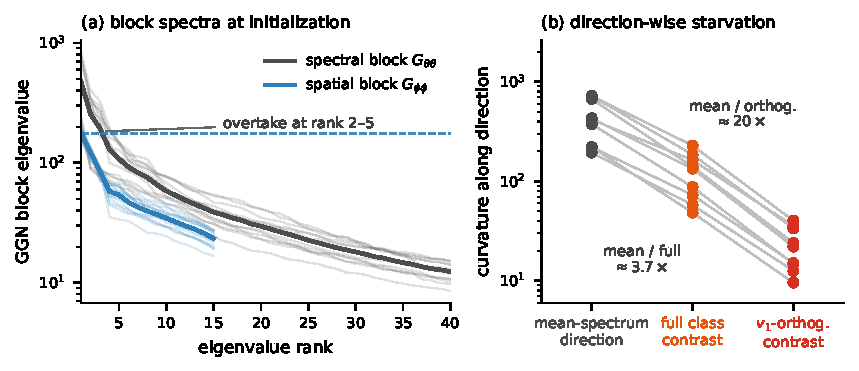
\includegraphics[width=\linewidth]{figures/fig8a_geometry.pdf}
\caption{Directional curvature anisotropy at initialization (breast
QCL, $M{=}192$, 3 seeds $\times$ 4 batches). (a)~GGN block eigenvalue
spectra: thin lines are individual measurements, thick lines their
means; the dashed line marks the spatial block's top eigenvalue, which
overtakes the spectral spectrum at rank $2$--$5$. (b)~Spectral
curvature along three input directions, for each of the nine
measurements whose batch contains both classes (3 seeds $\times$ 3
batches at $M{=}192$); thin grey lines join the three values of one
measurement. Left: the leading input direction $v_1$, i.e.\ the
mean-spectrum direction. Middle: the full, un-orthogonalized
CancerEpi--CAS class contrast, which retains its $v_1$ component
($|\cos(d, v_1)| = 0.45$). Right: that same contrast after
orthogonalization against $v_1$. Curvature is $3.7\times$ lower along
the full contrast than along $v_1$ (range $2.6$--$4.8\times$) and
$20\times$ lower along the $v_1$-orthogonalized contrast (range
$12$--$28\times$): the large anisotropy is a statement about the
$v_1$-orthogonal part of the contrast, not about the class contrast as
a whole.}
\label{fig:real_geometry}
\end{figure}

\paragraph{Normalization sets the cap.}
The cap is not an immutable property of the tissue: removing the
spectral normalization deflates $\lambda_{\max}(G_{\thetap\thetap})$ by
$2.4\times$ ($471 \to 194$ at $M{=}192$) and pushes the ratio across
parity ($1.18$ at $M{=}192$, $1.31$ at $M{=}384$). Input
\emph{centering}, by contrast, changes nothing when the architecture
contains internal batch normalization ($\mathcal{D}_{\mathrm{curv}}$ identical to three
decimals with and without centering): a linear projection followed by
normalization absorbs constant input shifts exactly. The lever on the
curvature geometry acts through the normalization choice, not the
preprocessing pipeline.

\subsection{Controlled retraining dynamics}
\label{sec:real_dynamics}

We train the pipeline ourselves on breast QCL (fold 0), at reduced
depth (6 transformer layers rather than the 12 of
Section~\ref{sec:real_setup}) and with full instrumentation. Two
protocols were run and we report both. The \emph{original protocol}
(39 runs) is the pre-registered one; an audit of the training code
afterwards found three incidental asymmetries between its arms, so its
joint-versus-frozen contrast is confounded. The \emph{matched
protocol} (21 runs) removes those asymmetries, saves the selected
checkpoint, and re-runs the pre-registered comparisons; it is the one
on which the conclusions of this subsection rest. In both protocols
per-step residuals, block gradient norms, and per-epoch parameter
displacements and input-Jacobian norms are recorded; the matched
protocol additionally logs the per-step clipping coefficient and the
per-block applied update norms. Sixty logged runs in total.

\paragraph{Original protocol, and why its comparison is not fair.}
Arms $\{$joint-linear, frozen-random, frozen-PCA, joint-MLP$\}$
$\times$ widths $M \in \{48, 192\}$ $\times$ 3 seeds under AdamW
(60 epochs), plus a $\{$joint-linear, frozen-random$\}$ $\times$
3-seed pair under momentum SGD at both widths and a frozen-PCA SGD
triple at $M{=}48$ as a positive control. Following
Section~\ref{sec:thm2}, the spectral parameters sit in a
zero-weight-decay group in every arm; frozen arms log counterfactual
spectral gradients. On the pre-registered metric --- mean validation
macro-F1 over the final 5 epochs --- the arm with the spectral module
frozen at a \emph{random} initialization scores higher than the jointly
trained arm at both widths under AdamW: the gaps are $-0.110$ at
$M{=}48$ ($90\%$ paired-$t$ interval $[-0.333, +0.114]$) and $-0.085$
at $M{=}192$ ($[-0.185, +0.015]$), neither of them resolvable at $n=3$
(Figure~\ref{fig:e3c}a, Table~\ref{tab:e3c}). The pre-registered
falsifier --- joint scoring above frozen-PCA --- is negative at both
widths ($-0.193$, $[-0.334, -0.052]$; $-0.081$, $[-0.175, +0.014]$).
Taking instead each run's maximum over its 60
per-epoch evaluations reverses the ordering: joint $-$ frozen-random
$= +0.033$ ($M{=}48$) and $+0.041$ ($M{=}192$), joint $-$ frozen-PCA
$= +0.104$ and $-0.004$. The switch between the two policies is an
arithmetic identity: the change in every gap is exactly the difference
in peak-to-final degradation between the two arms. Averaged over
seeds, that degradation is $0.335$ ($M{=}48$) and $0.212$ ($M{=}192$)
for joint-linear against $0.192$ and $0.086$ for frozen-random --- both
arms are far from convergence at epoch 60, and the joint arms give
back more of their peak.

Three asymmetries between the arms, identified after these runs were
complete, make the joint-versus-frozen contrast unfair rather than
merely noisy. First, gradient-norm clipping at $1.0$ is computed over
the optimizer's parameters, that is over $\thetap{+}\phip$ in the
joint arms but over $\phip$ alone in the frozen arms, so at identical
gradients the frozen arm takes the larger $\phip$ step: the median
extra clip factor paid by the joint arm is $1.10$--$1.12$ under SGD at
$M{=}48$ and $3.0$--$3.6$ under AdamW at $M{=}192$. Second, the batch
normalization following the spectral projection contributes $128$
affine parameters that are trained in joint-linear, frozen in
frozen-random, and structurally absent in frozen-PCA; parameter count
is not a defense, since normalization parameters can have large
functional effects. Third, no checkpoint was saved during training, so
the best-validation column is a post-hoc curve maximum that no saved
model realizes; it is additionally taken over 60 evaluations of the
same 28 validation cores that define the comparison, and this study
has no test set. We therefore report the ``frozen $>$ joint on the
final-window metric'' result as \emph{pre-registered but confounded}
--- it is what the registration asked for, measured as registered, on
a comparison whose arms differ in more than the registered factor ---
and the best-validation reanalysis as exploratory and
selection-optimistic by construction. Neither column licenses a
statement about which method deploys better.

\begin{table}[h]
\centering
\caption{Controlled study, \emph{original protocol}, AdamW arms:
validation macro-F1 (mean $\pm$ sd over 3 seeds) under two checkpoint
policies, and relative spectral-parameter displacement at end of
training. \emph{Final-5} is the pre-registered metric (mean over the
final 5 epochs). \emph{Best-val} is the maximum over the 60 per-epoch
evaluations on the same 28 validation cores; it is a post-hoc curve
maximum --- no test set exists in this study and no checkpoint was
saved at the maximum --- and is reported as exploratory and
selection-optimistic (see text). The two policies order the arms
oppositely. The arms of this protocol differ in clip scope and in
batch-normalization affine treatment as well as in the registered
factor; the fair comparison is Table~\ref{tab:e3c_matched}.}
\label{tab:e3c}
\small
\begin{tabular}{lccccr}
\toprule
& \multicolumn{2}{c}{Final-5 (pre-registered)} & \multicolumn{2}{c}{Best-val (exploratory)} & \\
\cmidrule(lr){2-3}\cmidrule(lr){4-5}
Arm & $M{=}48$ & $M{=}192$ & $M{=}48$ & $M{=}192$ & $\|\Delta\thetap\|/\|\thetap_0\|$ \\
\midrule
Joint (linear)  & $0.538 \pm 0.082$ & $0.646 \pm 0.050$ & $0.873 \pm 0.030$ & $0.858 \pm 0.056$ & $0.54$--$0.64$ \\
Frozen random   & $0.648 \pm 0.063$ & $0.731 \pm 0.023$ & $0.840 \pm 0.025$ & $0.817 \pm 0.017$ & $0$ \\
Frozen PCA      & $0.731 \pm 0.003$ & $0.726 \pm 0.012$ & $0.769 \pm 0.021$ & $0.862 \pm 0.068$ & $0$ \\
Joint (MLP)     & $0.566 \pm 0.070$ & $0.575 \pm 0.184$ & $0.900 \pm 0.000$ & $0.897 \pm 0.001$ & $0.85$--$0.96$ \\
\bottomrule
\end{tabular}
\end{table}

\begin{figure}[t]
\centering
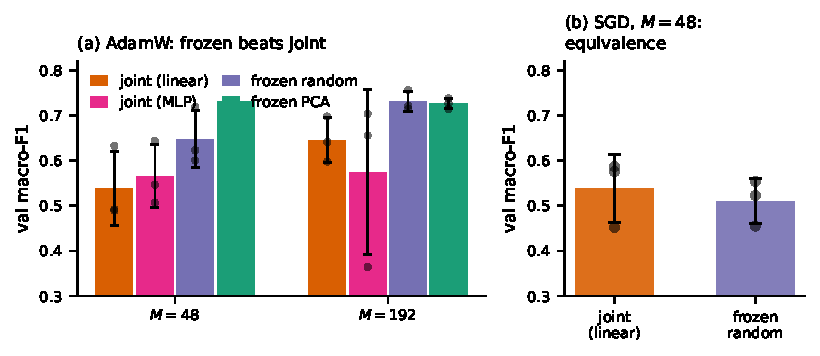
\includegraphics[width=\linewidth]{figures/fig8b_dynamics.pdf}
\caption{Controlled retraining study, \emph{original protocol} (breast
QCL fold 0; bars: mean over 3 seeds, whiskers: sd, dots: individual
seeds). (a)~Under AdamW, on the pre-registered final-window metric,
every frozen arm scores higher than every joint arm at both widths; the
ordering reverses under a best-validation policy (Table~\ref{tab:e3c}).
Both orderings are confounded by the clip-scope and
batch-normalization-affine asymmetries described in the text and do
not survive the matched protocol (Table~\ref{tab:e3c_matched}).
(b)~Under momentum SGD --- an optimizer-family control, not an
instantiation of Theorem~\ref{thm:twoscale}'s gradient flow --- joint
training and frozen-random show no resolvable best-validation
difference at $n=3$, while their final-window gaps differ in sign
between the two widths.}
\label{fig:e3c}
\end{figure}

\paragraph{Momentum-SGD controls.}
The two optimizer families constitute an \emph{optimizer-family
control}; the SGD arm is not an instantiation of
Theorem~\ref{thm:twoscale}'s gradient flow, and we do not present it as
one. It uses momentum $0.9$; weight decay $0.01$ on $\phip$ and $0$ on
$\thetap$; mini-batches of $4$ cores with reshuffling; and global
gradient-norm clipping at $1.0$, which binds on $73$--$89\%$ of steps.
Logged gradient norms are recorded before clipping, so the theory
quantities we plot are not the quantities the trajectory applied.
Under momentum SGD, joint training and frozen-random show no resolvable
best-validation difference: the paired gap is $+0.002$ at $M{=}48$ and
$+0.011$ at $M{=}192$, with $90\%$ paired-$t$ intervals
$[-0.008, +0.011]$ and $[-0.007, +0.030]$ ($n=3$). On the final-window
metric the same pairs give $+0.028$ and $-0.057$, with intervals
$[-0.173, +0.228]$ and $[-0.124, +0.010]$ --- gaps that differ in sign
between the two widths, and intervals an order of magnitude wider than
the effect they bracket. What this establishes is no resolvable
best-validation difference between joint and frozen arms at $n=3$
(intervals above) in under-fitted momentum-SGD controls, in which both
arms lose $0.12$--$0.22$ macro-F1 between their peak and their final
window. It does not establish broader functional equivalence, and it is
not a test of
Theorem~\ref{thm:twoscale}: that theorem bounds the displacement of
$\thetap$ along the joint trajectory, and says nothing about the
difference between that trajectory and a separately trained frozen
model. Descriptively, the spectral share of total squared gradient flow
drops from $\approx 0.94$ (AdamW joint) to $\approx 0.26$ (SGD joint).
The optimizer family is the variable that changes the outcome;
momentum, clipping, weight decay and adaptivity all differ between the
two families, so no single factor is isolated here.

\paragraph{Batch-normalization recalibration.}
One inexpensive alternative explanation for the joint arms'
peak-to-final decline is stale batch-normalization running statistics
under drifting features and small core batches. We test it directly:
on disposable copies of the final checkpoints, with all weights fixed,
we re-estimate the normalization running statistics on training data
only (29 batches) and re-evaluate. The recovered fraction of the joint
arms' peak-to-final drop is only $0.17$ at $M{=}48$ and $0.07$ at
$M{=}192$, so recalibration does not undo the decline. What it does
undo is the instability of the endpoint number: it repairs the two
collapsed joint checkpoints ($+0.24$ and $+0.15$ macro-F1) and shrinks
the seed standard deviation by roughly $3.7\times$, while leaving the
frozen arms essentially unchanged ($|\Delta| \le 0.02$, and
$\le 0.006$ for frozen-PCA, whose spectral stage carries no batch
normalization). Stale normalization statistics therefore explain the
\emph{variance} of the joint arms' final-epoch number, not the
degradation itself.

\paragraph{Matched protocol.}
The matched protocol equalizes the three asymmetries and re-runs the
pre-registered comparisons at $M{=}48$ (Table~\ref{tab:e3c_matched},
Figure~\ref{fig:e3c_matched}):
the reduction-stage
batch-nor\-mal\-i\-za\-tion affine parameters are placed in $\phip$ and
trained in \emph{every} arm; the clip norm at $1.0$ is computed over
$\phip$ only in \emph{every} arm; and the best-validation checkpoint is
saved. AdamW at learning rate $10^{-4}$, 60 epochs, 3 seeds, flip and
$90^\circ$-rotation augmentation on in all arms. The seven arms are
frozen-random; joint-linear; frozen-pretrained (the E3c MLP spectral
encoder pretrained on fold-0 training pixels); fine-tune-pretrained
(the same initialization with $\thetap$ trainable and zero weight
decay, with gradient flow to $\thetap$ verified from the logged update
norms); joint-linear with the spectral learning rate multiplied by
$0.1$ and by $10$; and joint-linear under a cosine schedule. Clipping
still binds --- the logged per-step clip coefficient averages
$0.33$--$0.57$ across arms --- but now identically in every arm, and
the logged applied update norms confirm that the spectral share of the
applied update tracks the multiplier ($0.02$, $0.17$ and $1.36$ times
the $\phip$ update norm for $\times 0.1$, $\times 1$ and $\times 10$).
Four disclosures. The pretrained encoder was selected by pixel
validation macro-F1 on the \emph{same} fold-0 validation cores the
runner later scores, which is a selection advantage for both
pretrained arms; it was pretrained with weight decay $0.01$ on
$\thetap$. Augmentation is on in all arms. Validation is 28 fold-0
cores and there is no test set, so the best-validation column remains a
maximum over 60 evaluations on the selection split --- it is now
realized by a saved checkpoint, but it is still exploratory and
selection-optimistic, and the final-5 column remains the pre-registered
metric.

\begin{table}[h]
\centering
\caption{Controlled study, \emph{matched protocol} ($M{=}48$, AdamW,
3 seeds, mean $\pm$ sd). Identical batch-normalization affine
treatment and identical $\phip$-only clip scope in every arm;
best-validation checkpoints saved. \emph{Final-5} (mean over the final
5 epochs) is the pre-registered metric; \emph{best-val} is the maximum
over the 60 per-epoch evaluations on the 28 fold-0 validation cores and
is exploratory and selection-optimistic --- no test set exists in this
study. The last column is relative spectral-parameter displacement at
end of training.}
\label{tab:e3c_matched}
\small
\begin{tabular}{lccr}
\toprule
Arm & Final-5 (pre-registered) & Best-val (exploratory) & $\|\Delta\thetap\|/\|\thetap_0\|$ \\
\midrule
Frozen random                     & $0.684 \pm 0.037$ & $0.814 \pm 0.040$ & $0$ \\
Joint (linear)                    & $0.694 \pm 0.056$ & $0.837 \pm 0.029$ & $0.57$ \\
Frozen pretrained                 & $0.690 \pm 0.033$ & $0.861 \pm 0.022$ & $0$ \\
Fine-tuned pretrained             & $0.710 \pm 0.052$ & $0.857 \pm 0.009$ & $0.02$ \\
Joint, spectral lr $\times 0.1$   & $0.626 \pm 0.055$ & $0.841 \pm 0.007$ & $0.08$ \\
Joint, spectral lr $\times 10$    & $0.561 \pm 0.114$ & $0.886 \pm 0.037$ & $4.91$ \\
Joint, cosine schedule            & $0.660 \pm 0.020$ & $0.825 \pm 0.033$ & $0.36$ \\
\bottomrule
\end{tabular}
\end{table}

\begin{figure}[t]
\centering
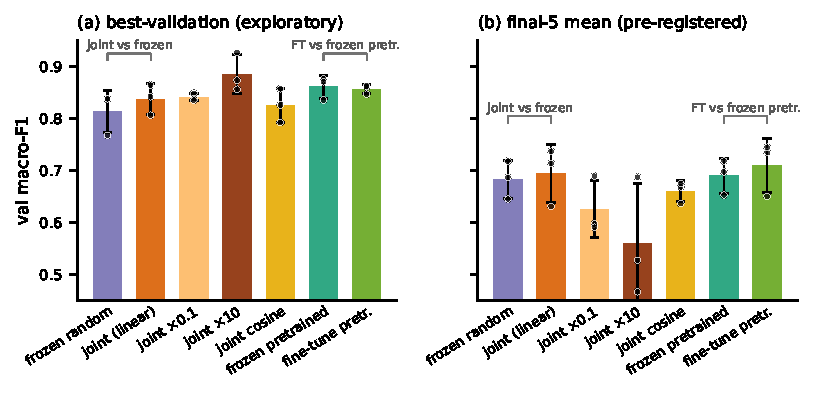
\includegraphics[width=\linewidth]{figures/fig8c_matched.pdf}
\caption{Controlled study, \emph{matched protocol}: identical
batch-normalization affine treatment, $\phip$-only clipping and saved
best-validation checkpoints in every arm ($M{=}48$, AdamW, 3 seeds;
dots are seeds, bars are seed means, whiskers sd). (a)~Best-validation
macro-F1 --- a post-hoc maximum over 60 evaluations on the same 28-core
fold-0 validation split, hence exploratory and selection-optimistic.
(b)~The pre-registered metric, the mean over the final 5 epochs.
Brackets mark the two pre-registered pairs; no pre-registered
difference is resolvable at $n=3$ under either policy.}
\label{fig:e3c_matched}
\end{figure}

\paragraph{The pre-registered predictions under the matched protocol.}
All comparisons below are paired by seed with $90\%$ $t$-intervals
($t = 2.920$, $n = 3$), conditional on this one validation split.

\emph{P1: fine-tuning a pretrained spectral encoder falls below leaving
it frozen.} Not supported. Fine-tune-pretrained $-$ frozen-pretrained
is $-0.004$ $[-0.048, +0.039]$ on best-val and $+0.021$
$[-0.022, +0.063]$ on final-5: no resolvable difference at $n=3$.
Fine-tuning with verified gradient flow to $\thetap$ matched the frozen
pretrained encoder within noise, and moved $\thetap$ by only $2\%$ of
its initial norm. The prediction is not supported; neither is it
refuted in the direction of fine-tuning helping.

\emph{Joint versus frozen at matched informativeness.} No resolvable
difference. Joint-linear $-$ frozen-random is $+0.023$
$[-0.066, +0.112]$ on best-val and $+0.011$ $[-0.142, +0.163]$ on
final-5. The original protocol's $M{=}48$ final-window deficit of
$-0.110$ is gone once the batch-normalization affine treatment and the
clip scope are equalized. Pretraining is directionally worth something
--- frozen-pretrained $-$ frozen-random is $+0.047$
$[-0.042, +0.136]$ on best-val --- but is unresolved at $n=3$, and the
pretrained arms carry the validation-selection advantage disclosed
above.

\emph{The spectral-learning-rate discriminator.} The pre-registered
harmful-drift prediction --- the ordering
$\times 0.1 \ge \times 1 \ge \times 10$ --- is not observed. On best-val
the ordering is reversed: $\times 10 - \times 1 = +0.048$
$[-0.016, +0.112]$, positive in $3/3$ seeds though not resolved at
$n=3$, while $\times 0.1 - \times 1 = +0.004$ $[-0.039, +0.046]$. On
final-5 the ordering is non-monotone, with both extremes below
$\times 1$: $\times 0.1 - \times 1 = -0.068$ $[-0.173, +0.037]$ and
$\times 10 - \times 1 = -0.133$ $[-0.419, +0.152]$. We report all three
points under both metrics and draw no binary mechanism verdict. The
cosine schedule helps on neither metric ($0.825$ best-val, $0.660$
final-5, against $0.837$ and $0.694$ for the constant learning rate),
so the late decline of the joint arms is not simply an
excessive-late-learning-rate effect.

\paragraph{Reading the matched results.}
Under a protocol whose arms differ only in the registered factor, at
$M{=}48$ with three seeds, neither a freezing benefit nor a freezing
penalty is resolvable: all four core arms lie between $0.81$ and $0.86$
best-val and between $0.68$ and $0.71$ final-5, with paired intervals
that straddle zero by margins several times the point estimates. What
does vary systematically with the spectral learning rate is the shape
of the trajectory rather than its quality at a fixed policy: larger
spectral movement raises the attainable peak (the $\times 10$ arm
drifts $\thetap$ by $4.9$ times its initial norm and attains the
highest best-val of any arm) and lowers the un-stopped endpoint (the
same arm has the lowest and by far the most variable final-5). We read
this as a checkpoint-policy trade-off, and it selects neither of the
two pre-registered mechanism readings: the $\times 0.1$ arm, which the
pre-registered starvation prediction would penalize and the
pre-registered harmful-drift prediction would favor, is unresolved
against $\times 1$ on best-val and below it on final-5. Two further
cautions carry over. A large parameter displacement is not by itself
evidence that spectral information was lost --- a linear projection can
change scale or basis substantially while spanning much the same
subspace, and such changes are compensable by the downstream
normalization and the spatial module --- and we have not measured the
features: subspace-overlap and linear-decodability probes of the
learned spectral representation are pending, so displacement remains a
description of the trajectory rather than a diagnosis of it. Taken
together with the original-protocol result, the conclusion we draw
from this subsection is that \emph{the measurable shortcut on this
pipeline is a property of the training protocol, not of the
architecture}: clip scope, normalization-parameter placement and
checkpoint policy were sufficient to manufacture a
$0.11$ macro-F1 freezing advantage that disappears when they are
equalized. This is stated for $M{=}48$, $n=3$ seeds, a single
validation-selected fold and no test set; it does not extend to the
production widths of Section~\ref{sec:real_observation}, whose
comparison remains an observation we have not reproduced under matched
hygiene.

\paragraph{Envelope curvature grows with width.}
The fitted residual-envelope rate for the joint-linear arm, expressed
per optimizer step, grows from $\hat\mu = 6.0 \times 10^{-4}$
($M{=}48$) to $1.9 \times 10^{-3}$ ($M{=}192$), a factor $3.2$ for a
$4\times$ width increase. The ratio is invariant to the
step-clock-to-flow-time conversion discussed in
Section~\ref{sec:real_scope}; the absolute values are not. This is
directionally consistent with a width-growing NTK rate of the kind
Proposition~\ref{prop:ntk_classprior} describes, but it is not a test
of that proposition: the proposition assumes the same dense-head
hypothesis this architecture does not meet
(Section~\ref{sec:real_setup}), and two widths do not establish a
trend.

\paragraph{The scalar EGR diagnostic is blind here.}
The scalar effective-gradient-ratio \emph{rises} during joint AdamW
training (joint-linear epoch-1 median $0.6$--$0.8$, rising to $3$--$5$
by epoch 60), including in the runs whose validation score is falling. A single
global ratio cannot see a direction-wise anisotropy (cf.\
Remark~\ref{rem:egr_ratio_caveat}): the spectral gradients are large
along the mean-spectrum direction and small along the discriminative
ones, consistent with the initialization geometry of
Section~\ref{sec:real_geometry}. Direction-resolved diagnostics are
future work, and they are what would turn the anisotropy hypothesis of
Section~\ref{sec:real_geometry} into a test.
% TODO(P5): appendix figure — EGR trajectories + envelope fit example.

\subsection{What the theorems do and do not predict here}
\label{sec:real_scope}

Honest scoping of the quantitative statements. The spatial module's
input-Jacobian operator norm grows by orders of magnitude over training
($3.2 \to 157$ on average for joint-linear, up to $414$;
$1.7 \to 1.2 \times 10^{4}$ for joint-MLP). This rejects an
initialization-scale stability approximation for the containment
constant of Theorem~\ref{thm:twoscale}, though it does not refute the
existence of a finite-horizon constant over the training window.

We do not obtain a useful certified bound for the production regime. A
proxy instantiation of the theorem's displacement bound --- a per-step
envelope fitted to a 25-step smoothed mini-batch residual, a
99th-percentile rather than supremum gain, and no conversion from the
optimizer's step clock to flow time --- exceeds the measured
displacement by $2 \times 10^{4}$--$2 \times 10^{5}$. Correcting the
time units ($\hat\mu_{\mathrm{flow}} = \hat\mu_{\mathrm{step}}/\eta$)
and using
the supremum gain, the proxy still exceeds the measured displacement by
$\approx 17$--$47\times$ under AdamW and $\approx 450$--$1900\times$
under momentum SGD; and the raw per-step residual violates the fitted
envelope on $19$--$28\%$ of the joint-linear steps, so the
residual-envelope assumption is verified for the smoothed curve rather
than for the logged quantity.
None of these figures is a certified instantiation of
Theorem~\ref{thm:twoscale}. Momentum, gradient clipping and adaptive
preconditioning all lie outside its hypotheses, and under AdamW the
measured displacement exceeds
$\eta \sum_k \|\nabla_{\thetap}\loss_k\|$ by more than an order of
magnitude, so no $\eta$-rescaled flow bound describes that trajectory
in either direction. No certified instantiation exists for this
pipeline at present.

The synthetic setting of Section~\ref{sec:experiments}, where
containment holds by construction, is where the bound is quantitatively
informative. On real data the theory's contribution is narrower. Two of
its ingredients are measured directly here: a width-independent
spectral cap, and a width-growing --- though sublinear, and not
guaranteed for this architecture --- spatial curvature. The class-prior
NTK floor of Proposition~\ref{prop:ntk_classprior} was not measured on
this model, and its head hypothesis is not met by this architecture, so
it is neither verified nor available as an explanation here. And the
regime-resolved dynamics above are an optimizer-family control rather
than a confirmation of the theorem inside its own regime. Nothing here
establishes that spectral drift is harmful: the pre-registered
learning-rate discriminator did not produce the ordering that reading
predicts (Section~\ref{sec:real_dynamics}), and the association between
larger spectral movement and a lower un-stopped endpoint is reported as
a checkpoint-policy trade-off, not as a demonstrated mechanism.

One scoping statement concerns the empirical headline rather than the
theory. Under the matched protocol of
Section~\ref{sec:real_dynamics}, the practical claim that freezing the
spectral module is better than training it does not survive: at
$M{=}48$, with $n=3$ seeds and a validation-selected checkpoint, no
freezing benefit
or penalty is resolvable. What remains from the controlled study is a
diagnostic-limits result --- which of the theory's ingredients can and
cannot be measured to constrain anything on a production pipeline ---
together with the demonstration that incidental protocol asymmetries
(clip scope, normalization-parameter placement, checkpoint policy) are
by themselves sufficient to manufacture an apparent freezing effect of
the size reported in the literature.

The companion study \citep{dziuba2026spatial} additionally provides a
pixel-level tokenization benchmark across three datasets and the
spatial-transfer experiment on breast QCL from which
Table~\ref{tab:real} is drawn; those results characterize \emph{what}
performs well, while the present analysis asks \emph{why} end-to-end
training of the spectral stage may underperform, and how far the
present theory can account for it.
